\section{Figures}\label{figures}

\begin{figure}
\centering
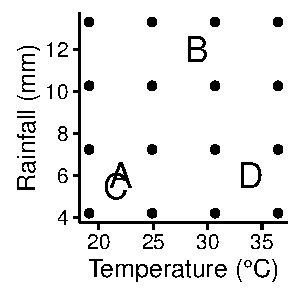
\includegraphics{figures_files/figure-latex/unnamed-chunk-3-1.pdf}
\caption{Attribute space example. This environmental attribute space has
dimensions relating to annual temperature (\(^{\circ}\)C) and rainfall
(mm). Letters denote the environmental conditions associated with the
geographic locations where four hypothetical populations are found.
Points represent demand points. In this space, populations close to each
other inhabit similar environmental conditions.}
\end{figure}

\begin{figure}
\centering
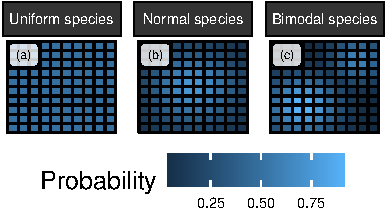
\includegraphics{figures_files/figure-latex/unnamed-chunk-4-1.pdf}
\caption{Distributions of three simulated species. Squares denote
planning units. Colors indicate probability of occupancy.}
\end{figure}

\begin{figure}
\centering
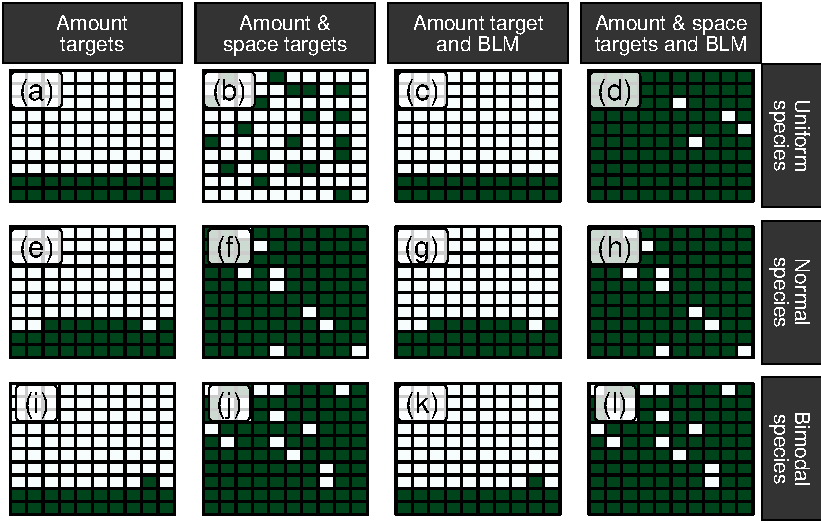
\includegraphics{figures_files/figure-latex/unnamed-chunk-5-1.pdf}
\caption{Prioritizations for the simulation study. Each panel shows a
prioritization generated for a single species using a set of parameters.
Squares denote planning units. Dark green planning units were selected
for protection. Each row of panels show prioritizations generated for a
different species. Each column of panels corresponds to a different set
of parameters used to generate the prioritization.}
\end{figure}

\begin{figure}
\centering
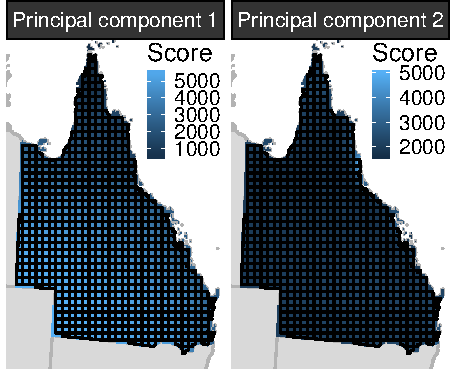
\includegraphics{figures_files/figure-latex/unnamed-chunk-6-1.pdf}
\caption{Two main gradients of climatic variation across Queensland,
Australia. Polygons denote planning units.}
\end{figure}

\begin{figure}
\centering
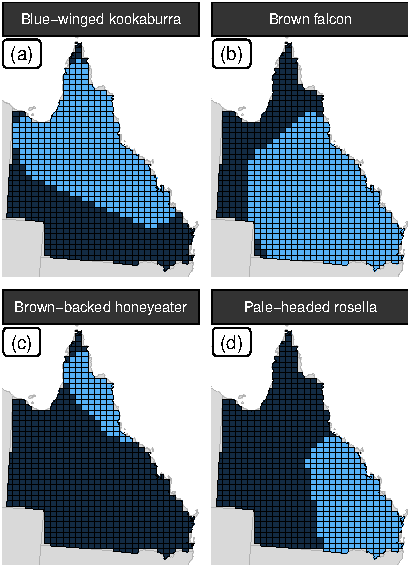
\includegraphics{figures_files/figure-latex/unnamed-chunk-7-1.pdf}
\caption{Distribution of the species used in the first case study.
Polygons denote planning units. Planning units occupied by a given
species are shown in light blue.}
\end{figure}

\begin{figure}
\centering
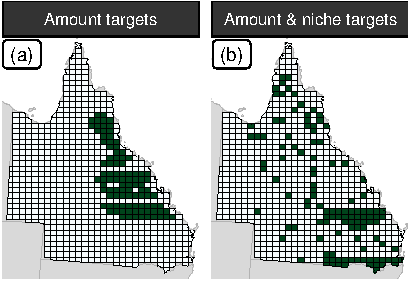
\includegraphics{figures_files/figure-latex/unnamed-chunk-8-1.pdf}
\caption{Prioritizations for the first case study. Polygons denote
planning units. Dark green planning units were selected for protection.
Panel (a) shows the solution generated when using 20 \% amount targets.
Panel (b) shows the solution when using 20 \% amount targets and -1e+06
\% niche targets.}
\end{figure}

\begin{figure}
\centering
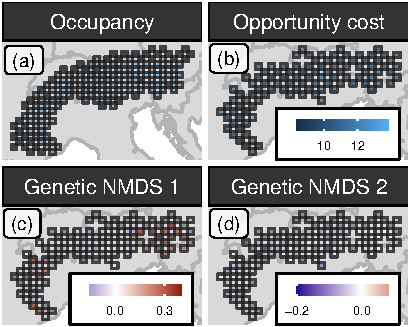
\includegraphics{figures_files/figure-latex/unnamed-chunk-9-1.pdf}
\caption{Data used for the second case study. Squares denote planning
units. Panel (a) shows all grid cells surveyed by the IntraBioDiv
project. Grid cells occupied by the betony-leaved rampion are shown in
bright blue. The subsequent panels contain only show occupied grid
cells. Panel (b) shows the acquisition cost of each planning unit
(estimated as the total human population density). Panels (c--d) show
the spatial distribution of the ordinations describing genetic
variation. These values describe the typical genetic characteristics of
individuals in each planning unit. Planning units with similar
values/colors contain individuals with similar loci polymorphisms.}
\end{figure}

\begin{figure}
\centering
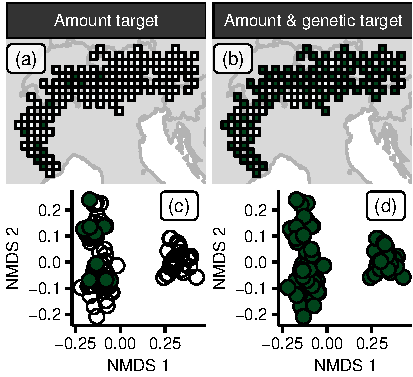
\includegraphics{figures_files/figure-latex/unnamed-chunk-10-1.pdf}
\caption{Prioritizations for the second case study. Panels (a--b) show
prioritizations generated using different parameters. Polygons denote
planning units. Dark green planning units were selected for protection.
Panel (a) shows the planning units selected when using 10 \% amount
targets. Panel (b) shows the planning units selected when using \%
amount targets and 85 \% genetic targets. Panels (c--d) show the
solutions in the genetic space. Each point corresponds to a planning
unit. The coordinates of the points represent the typical genetic
characteristics of individuals sampled in that planning unit (based on
an NMDS of the binary loci data). Planning units associated with points
that are closer together contain individuals with more similar genetic
characteristics than planning units that are further apart.}
\end{figure}
